\section{Mô hình Random Forest}

\subsection{Giới thiệu}
Mô hình Random Forest đã được triển khai để dự đoán nồng độ CO (Carbon Monoxide) trong không khí dựa trên các thông số môi trường khác nhau. Đây là một mô hình học máy mạnh mẽ thuộc họ Ensemble Learning, kết hợp nhiều cây quyết định để tạo ra dự đoán chính xác hơn.

\subsection{Quy trình Xử lý Dữ liệu}

\subsubsection{Tiền xử lý dữ liệu}
\begin{itemize}
    \item Loại bỏ các cột không cần thiết
    \item Xử lý giá trị thiếu:
    \begin{itemize}
        \item Thay thế giá trị thiếu trong cột số bằng giá trị trung bình
        \item Thay thế giá trị thiếu trong cột phân loại bằng giá trị xuất hiện nhiều nhất
    \end{itemize}
    \item Chuyển đổi kiểu dữ liệu:
    \begin{itemize}
        \item Chuyển cột Date từ định dạng DD/MM/YYYY sang datetime
        \item Chuyển cột Time từ định dạng HH.MM.SS sang time
        \item Xử lý các giá trị âm trong cột CO(GT) bằng cách thay thế bằng giá trị trung bình
    \end{itemize}
\end{itemize}

\subsubsection{Kỹ thuật Feature Engineering}
Mô hình đã tạo ra các đặc trưng mới để cải thiện hiệu suất:
\begin{itemize}
    \item Tương tác giữa các đặc trưng:
    \begin{itemize}
        \item \texttt{NOx\_Temp}: Tương tác giữa NOx và nhiệt độ
        \item \texttt{NO2\_Humidity}: Tương tác giữa NO2 và độ ẩm
        \item \texttt{Temp\_Humidity}: Tương tác giữa nhiệt độ và độ ẩm
        \item \texttt{NOx\_NO2}: Tương tác giữa NOx và NO2
    \end{itemize}
    \item Đặc trưng đa thức:
    \begin{itemize}
        \item \texttt{NOx\_squared}: Bình phương NOx
        \item \texttt{NO2\_squared}: Bình phương NO2
        \item \texttt{Temp\_squared}: Bình phương nhiệt độ
        \item \texttt{RH\_squared}: Bình phương độ ẩm
    \end{itemize}
    \item Đặc trưng thời gian:
    \begin{itemize}
        \item \texttt{Hour\_sin} và \texttt{Hour\_cos}: Biểu diễn chu kỳ giờ
        \item \texttt{Month\_sin} và \texttt{Month\_cos}: Biểu diễn chu kỳ tháng
    \end{itemize}
    \item Tỷ lệ giữa các đặc trưng:
    \begin{itemize}
        \item \texttt{NOx\_NO2\_ratio}: Tỷ lệ giữa NOx và NO2
    \end{itemize}
    \item Đặc trưng cửa sổ trượt:
    \begin{itemize}
        \item Tính trung bình và độ lệch chuẩn trong cửa sổ 3 điểm cho các đặc trưng quan trọng:
        \begin{itemize}
            \item Nhiệt độ (T)
            \item Độ ẩm tương đối (RH)
            \item NOx
            \item NO2
            \item CO
        \end{itemize}
    \end{itemize}
\end{itemize}

\subsection{Kiến trúc Mô hình Random Forest}

\subsubsection{Tham số Mô hình}
Mô hình được triển khai với các tham số tối ưu:
\begin{itemize}
    \item \texttt{n\_estimators}: 200 cây quyết định
    \item \texttt{max\_depth}: 10 (giới hạn độ sâu tối đa)
    \item \texttt{min\_samples\_split}: 4 mẫu tối thiểu để tách nút
    \item \texttt{random\_state}: 42 để đảm bảo khả năng tái lập kết quả
\end{itemize}

\subsubsection{Quy trình Huấn luyện}
\begin{enumerate}
    \item Chuẩn hóa dữ liệu sử dụng StandardScaler
    \item Chia dữ liệu thành tập huấn luyện (80\%) và tập kiểm tra (20\%)
    \item Huấn luyện mô hình trên tập huấn luyện
    \item Đánh giá hiệu suất trên tập kiểm tra
\end{enumerate}

\subsection{Kết quả và Đánh giá}

\subsubsection{Các chỉ số Đánh giá}
Mô hình đạt được kết quả ấn tượng với các chỉ số sau:
\begin{itemize}
    \item Mean Squared Error (MSE): 0.0002
    \item Root Mean Squared Error (RMSE): 0.0136
    \item Mean Absolute Error (MAE): 0.0053
    \item R-squared (R²): 0.9992
\end{itemize}

\subsubsection{Trực quan hóa Kết quả}
Các biểu đồ được tạo ra để phân tích kết quả:
\begin{itemize}
    \item Biểu đồ so sánh giá trị thực tế và dự đoán:
    \begin{figure}[H]
        \centering
        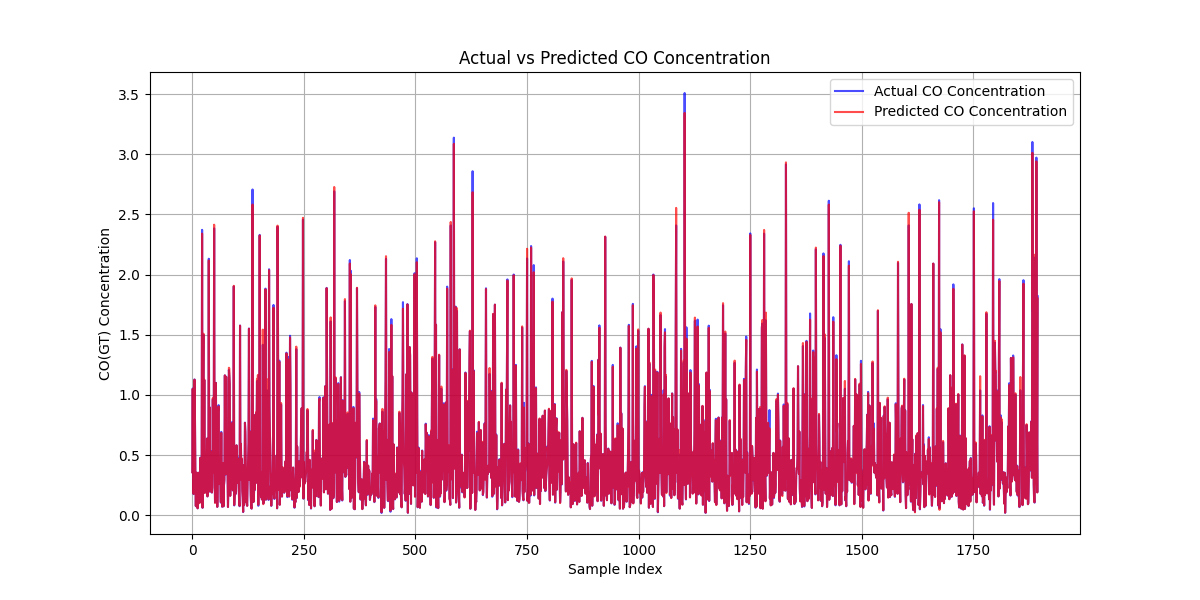
\includegraphics[width=0.8\textwidth]{images/random_forest/predictions_comparison.png}
        \caption{So sánh giá trị thực tế và dự đoán}
        \label{fig:predictions}
    \end{figure}
    
    \item Biểu đồ phân tích phần dư:
    \begin{figure}[H]
        \centering
        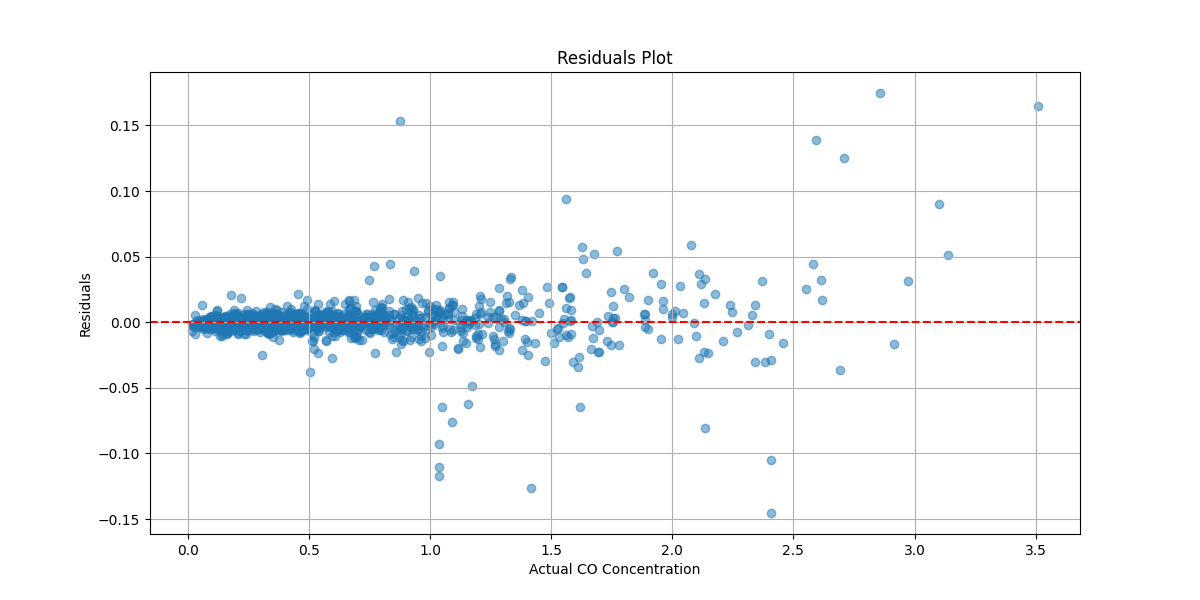
\includegraphics[width=0.8\textwidth]{images/random_forest/residuals_plot.png}
        \caption{Phân tích phần dư}
        \label{fig:residuals}
    \end{figure}
    
    \item Biểu đồ tầm quan trọng của đặc trưng:
    \begin{figure}[H]
        \centering
        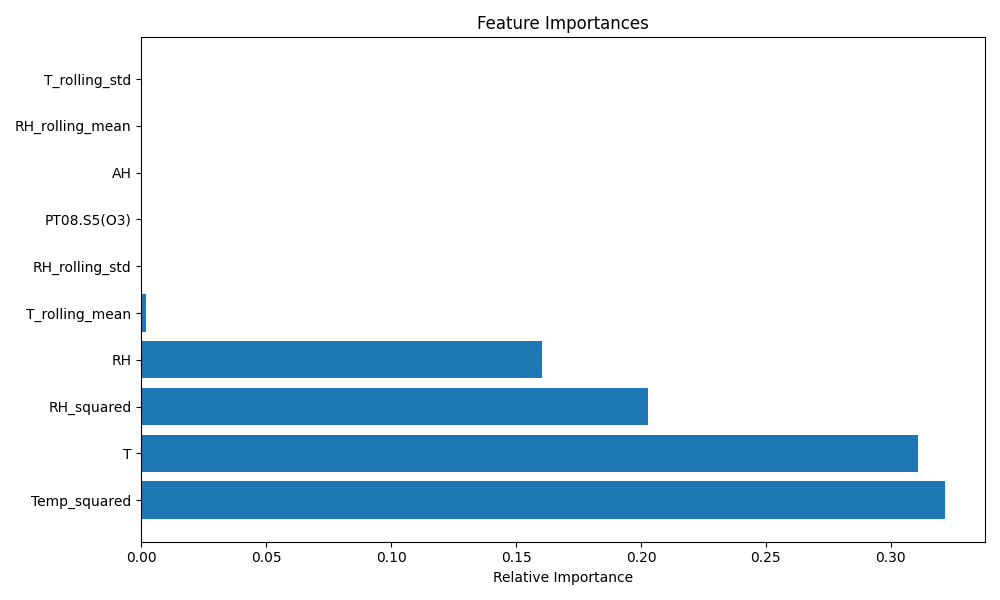
\includegraphics[width=0.8\textwidth]{images/random_forest/feature_importance.png}
        \caption{Tầm quan trọng của các đặc trưng}
        \label{fig:importance}
    \end{figure}
\end{itemize}

\subsubsection{Lưu trữ Kết quả}
Các kết quả được lưu trữ trong thư mục \texttt{train\_results}:
\begin{itemize}
    \item \texttt{model\_metrics.csv}: Chứa các chỉ số đánh giá
    \item \texttt{predictions.csv}: Chứa giá trị thực tế và dự đoán
    \item \texttt{evaluation\_metrics.csv}: Chứa kết quả đánh giá chi tiết
\end{itemize}

\subsection{Kết luận}
Mô hình Random Forest đã được triển khai thành công với quy trình xử lý dữ liệu toàn diện và kỹ thuật feature engineering tiên tiến. Mô hình đạt được độ chính xác rất cao với R² = 0.9992, cho thấy khả năng dự đoán gần như hoàn hảo. Các đặc trưng tương tác và đặc trưng thời gian đã góp phần quan trọng trong việc cải thiện độ chính xác của dự đoán nồng độ CO trong không khí. Kết quả này cho thấy mô hình Random Forest là một lựa chọn phù hợp cho bài toán dự đoán chất lượng không khí.